\documentclass[main.tex]{subfiles}

\begin{document}

\textcolor{red}{Лекция 26.03.2022.}

\section{Пороупругость}

Самый важный геомеханический раздел в контексте разработки месторождений.

Вспомним полученное ранее замыкающее соотношение на тензор \textbf{полных} напряжений \eqref{StressTens} (пусть нет начальных напряжений): 
\beq\label{PoroElast1}
T_{ij}=\overbrace{L_{ijkl}\varepsilon_{kl}}^{\substack{\text{эффективные}\\\text{напряжения}}}-\underbrace{\alpha_{ij}\left(p-p_0\right)}_{\substack{\text{пороупругая}\\\text{часть}}}-\overbrace{\alpha_{kl}^{\theta}L_{ijkl}\left(\theta-\theta_0\right)}^{\substack{\text{термические}\\\text{напряжения}}}
\eeq

Вспомним полученное ранее замыкающее соотношение на пористость \eqref{PhiConsRel}:
\beq\label{PoroElast2}
\varphi-\varphi_0=\alpha_{ijkl}\varepsilon_{ij}+\frac{p-p_0}{N}+\alpha_\theta^\varphi\left(\theta-\theta_0\right)
\eeq

Сейчас положительными считаем растягивающие напряжения.

Эффективные напряжения не равны скелетным напряжениям.

\subsection{Изотропный случай}
Перепишем равенство \eqref{PoroElast1}:
\beq
T_{ij}=\overbrace{K\varepsilon_{kk}\delta_{ij}+2G\left(\varepsilon_{ij}-\frac{1}{3}\varepsilon_{kk}\delta_{ij}\right)}^{\text{эффективные напряжения}}-\alpha \left(p-p_0\right)\delta_{ij}-3\alpha^{\theta}K\left(\theta-\theta_0\right)\delta_{ij}
\eeq

Перепишем равенство \eqref{PoroElast2}:
\beq
\varphi-\varphi_0=\alpha\varepsilon_{kk}+\frac{p-p_0}{N}+\alpha_\theta^\varphi\left(\theta-\theta_0\right)
\eeq

Связь между полной деформацией и деформацией скелета:
\beq
\varepsilon_{ij}=\left(1-\varphi\right)\varepsilon_{ij}^s+\left(\varphi-\varphi_0\right)\delta_{ij}
\eeq
Связь между полным напряжением и напряжением скелета:
\beq
T_{ij}=\left(1-\varphi\right)\sigma_{ij}^s-\varphi p\delta_{ij}
\eeq

\begin{figure}[h]
\centering
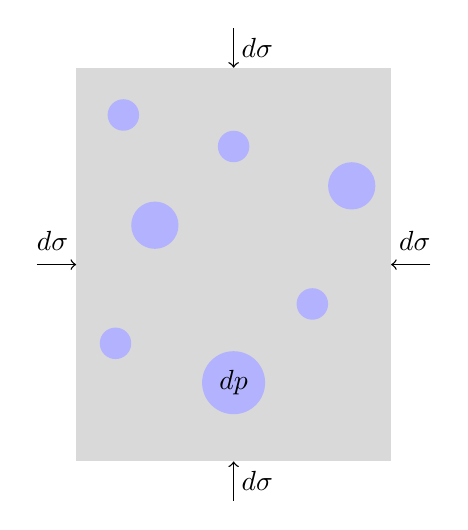
\begin{tikzpicture}[line width=0.5]
\fill[gray!30!white] (1,1) rectangle (5,6);
%\draw[gray] (1,1) -- (5,1) -- (5,6) -- (1,6) -- (1,1);
\fill[blue!30!white] (3,2) circle (0.4cm);
\node at (3,2) {$dp$};
\fill[blue!30!white] (4,3) circle (0.2cm);
\fill[blue!30!white] (2,4) circle (0.3cm);
\fill[blue!30!white] (3,5) circle (0.2cm);
\fill[blue!30!white] (1.6,5.4) circle (0.2cm);
\fill[blue!30!white] (4.5,4.5) circle (0.3cm);
\fill[blue!30!white] (1.5,2.5) circle (0.2cm);
\draw [->] (5.5,3.5) -- (5,3.5);
\node at (5.3,3.8) {$d\sigma$};
\draw [->] (3,0.5) -- (3,1);
\node at (3.3,0.75) {$d\sigma$};
\draw [->] (0.5,3.5) -- (1,3.5);
\node at (0.7,3.8) {$d\sigma$};
\draw [->] (3,6.5) -- (3,6);
\node at (3.3,6.25) {$d\sigma$};
\end{tikzpicture}
\caption{Пористый материал под нагрузкой}
\end{figure}
\newpage
Если $\alpha=\varphi$, то модуля Био не существует.

\end{document}